% Chapter 3

\chapter{\uppercase{SYSTEM DESIGN}} % Main chapter title
\label{ch:chap3} % For referencing
This chapter deals with the overall architecture of the system and description about each modules.
\section{\uppercase{OVERALL DESIGN AND DESCRIPTION}}
Figure \ref{fig:arch} gives the overall system design of this project.This project implements the following modules:

\begin{enumerate}
\item Control Flow Graph(CFG) Generator
\item Branch Appender
\item KLEE tool
\item User interface
\end{enumerate}

The input to the system involves a reference implementation that is the correct program without any logical errors, user implementation that is to be diagnosed for logical errors,constraints on the domain of involved inputs for functions involved in the program. 
The input given through user interface is used by the backend of the application to generate a new source file that follows specification for usage of KLEE.
The Branch Appender module takes the generated source file as input and produces a transformed source file wherein branch numbers  are appended to control flow branches.
The transformed source file is used by CFG Generator to generate a Control Flow Graph of both user and reference implementation .
KLEE is used to generate test cases on transformed source file and errored testcases are found by asserting that the return values of user and reference implementation are equal. The transformed source file is then with the failed testcases to print the branches taken by user and reference implementation for failed testcase. 

The output from the system involves a Control Flow Graph of both the user and reference implementation,test case for which the user implementation does not give expected output,branches taken by user and reference implementaion for the failed testcase.




\begin{figure}[h]
\centering
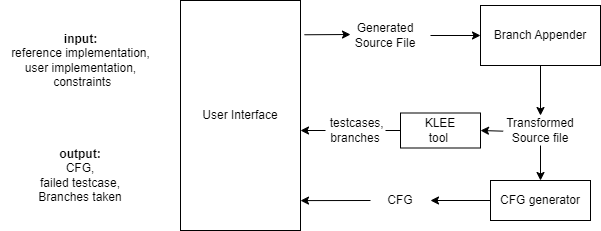
\includegraphics[width=1\textwidth]{3/systemarchi.png}
\caption{Architecture Diagram }
\label{fig:arch}
\end{figure}


\subsection{CONTROL FLOW GRAPH GENERATOR}

Clang is a C/C++/Objective-C compiler front-end. It is a sub-project of LLVM and uses LLVM for code optimization and back-end support. LLVM is a set of compiler and toolchain technologies that can be used to develop a front end for any programming language and a back end for any instruction set architecture. LLVM is designed around a language-independent intermediate representation (IR) that serves as a portable, high-level assembly language that can be optimized with a variety of transformations over multiple passes.Figure \ref{fig:llvm} shows how source code, clang, LLVM IR and LLVM are connected.

\begin{figure}[h]
\centering
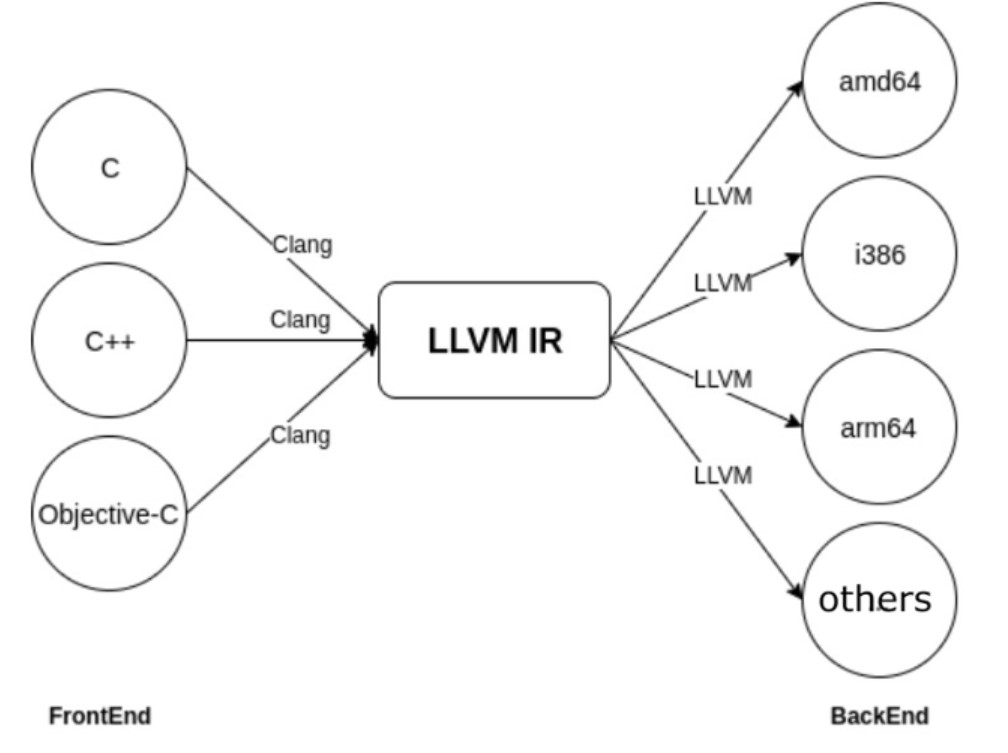
\includegraphics[width=1\textwidth]{3/llvm.jpg}
\caption{Structure of clang/llvm compiler}
\label{fig:llvm}
\end{figure}
Clang provides different interfaces that we can choose from to write a clang-tool. LibTooling is a library to support writing standalone tools based on Clang using which this module is implemented.Constructions of CFG procceds as follows using the above library :  Locating function declarations in the code by identifying nodes representing them in AST(Abstract Syntax Tree) generated by Clang,Accessing AST-Clang holds AST nodes in ASTContext which is defined in ASTContext.h. Clang’s library has prepared an abstract interface, ASTConsumer, which is defined in ASTConsumer.h. We have to define a new object that inherits ASTConsumer,  Reading AST-ASTConsumer has many methods for reading the AST. We are using HandleTranslationUnit (clang::ASTContext&) which is invoked when AST of each translation unit is parsed. This method is empty and we must override it, clang::ast\_matchers::MatchFinder class checks if there is a "matching node" in the context or not, clang::ast\_matchers::MatchFinder:: MatchCallback is a "callback" object which is called when the “matching node” that is registered for it is successfully found in the AST. “Finder” calls this method and passes the information of the “matching node” as an argument with type const \hspace{20} clang::ast\_matchers::MatchFinder::
MatchResult to it, The run function in callback object uses clang::CFG::buildCFG to finally construct the CFG.


\begin{figure}[h]
\centering
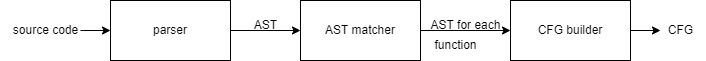
\includegraphics[width=1\textwidth]{3/ast.png}
\caption{Steps for generation of control flow graph (CFG)}
\label{fig:ast}
\end{figure}

\subsection{BRANCH APPENDER}
This Module takes as input the surce file that is generated by the Flask backend and appends print statements that print branch number for corresponding if/else/switch/while/for subblocks.

The source file is parsed by MyFrontEndAction which is a subclass of ASTFrontendAction by overriding  EndSourceFileAction() to create a copy Abstract Syntax Tree(AST) an instance of MYASTConsmer is created which is a subclass of ASTConsumer wherein HandleTopLevelDecl() is overriden to traverse the declarations iteratively and pass them to MyASTVisitor which is a subclass of RecursiveASTVisitor where VisitStmt() is overriden to append siblings in AST - 
 that is to append print branch statements to  if/else/switch/while/for subblocks.

\begin{figure}[h]
\centering
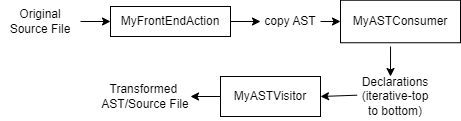
\includegraphics[width=1\textwidth]{3/branchappender.png}
\caption{Branch Appender Module}
\label{fig:graph_compare}
\end{figure}










\subsection{KLEE}
  
A dynamic symbolic execution engine built on top of the LLVM compiler infrastructure is used to automatically generate tests that achieve high coverage on a diverse set of complex and environmentally-intensive program.
  
Dynamic symbolic execution (DSE) is a well-known technique
for automatically generating tests to achieve higher levels of coverage in a program. Two keys ideas of DSE are to seed symbolic execution by executing a program on an initial input and using concrete values from the program execution in place of symbolic expressions whenever symbolic reasoning is hard or not desired.

Its step comprise of Identifying the code under test P and the symbolic inputs to P,Tracing the control flow path p taken by execution reinterpreting program operations to compute symbolic expressions,Generating a path-condition from p and the symbolic expressions,Generating a new input i by negating part of the path-condition, translating the path-condition to the input language of an ATP which stands for automated theorem prover which is a  computer program that show that some statement  is a logical consequence of a set of statements the axioms , invoking the ATP, and lifting a satisfying model back up to the source level,Guiding the search to expose new paths.

 

\begin{figure}[h]
\centering
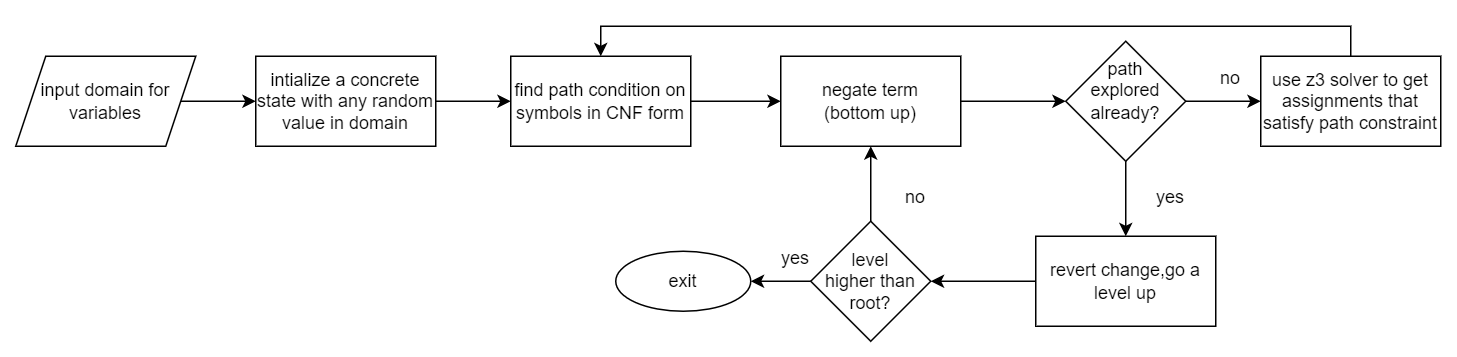
\includegraphics[width=1\textwidth]{3/k.png}
\caption{Dynamic Symbolic Execution procedure}
\label{fig:path}
\end{figure}

\subsection{USER INTERFACE}

The user interface uses jinja2 templates for frontend and flask for backend.The necessary headers,user program,reference program,argument type and constraints are received from the user.The Flask Backend creates new source file and appends these in correct format.shell scripts included in the backend are used to run cfg generator ,branch appender and klee tool  automatically using python's os.system() command .The resultant failed testcase,branches visited in that testcase,and the CFG for both the programs are displayed to the user.















